\documentclass{article}
\usepackage[utf8]{inputenc}
\usepackage{graphicx}
\graphicspath{ {images/} }
\usepackage{amsmath}
\usepackage{gensymb}
\usepackage[english]{babel}
\usepackage[version=4]{mhchem}
\usepackage[T1]{fontenc}
\usepackage{wrapfig}
\usepackage[colorlinks,citecolor=blue,urlcolor=blue,linkcolor=blue, bookmarks=false,hypertexnames=true]{hyperref} 
\usepackage[font=scriptsize,labelfont=bf]{caption}
\usepackage{subcaption}
\usepackage[backend=biber,style=authoryear-comp]{biblatex}
\usepackage[a4paper, portrait, margin=1in]{geometry}
\addbibresource{mybib_stable.bib}

\setlength{\parindent}{4em}
\setlength{\parskip}{1em}
\renewcommand{\baselinestretch}{1.5}

% \title{GIS For Dummies: Live Demonstration Guide}
% \author{Nicholas D. Barber}
% \date{\today}

\begin{document}

\begin{titlepage}
   \begin{center}
       \vspace*{1cm}

       \LARGE
       \textbf{GIS For Dummies: Session 2 Live Demo Guide}
       
       \Large
       \vspace{0.3cm}
        GIS Workshop prepared for McGill University Society for Economic Geology Student Chapter
            
       \vspace{1.2cm}
       \textbf{Nicholas D. Barber}\\
       Department of Earth Science\\
       University of Cambridge\\
       United Kingdom\\
       June 22nd, 2020
            
       \vspace{0.8cm}
     
       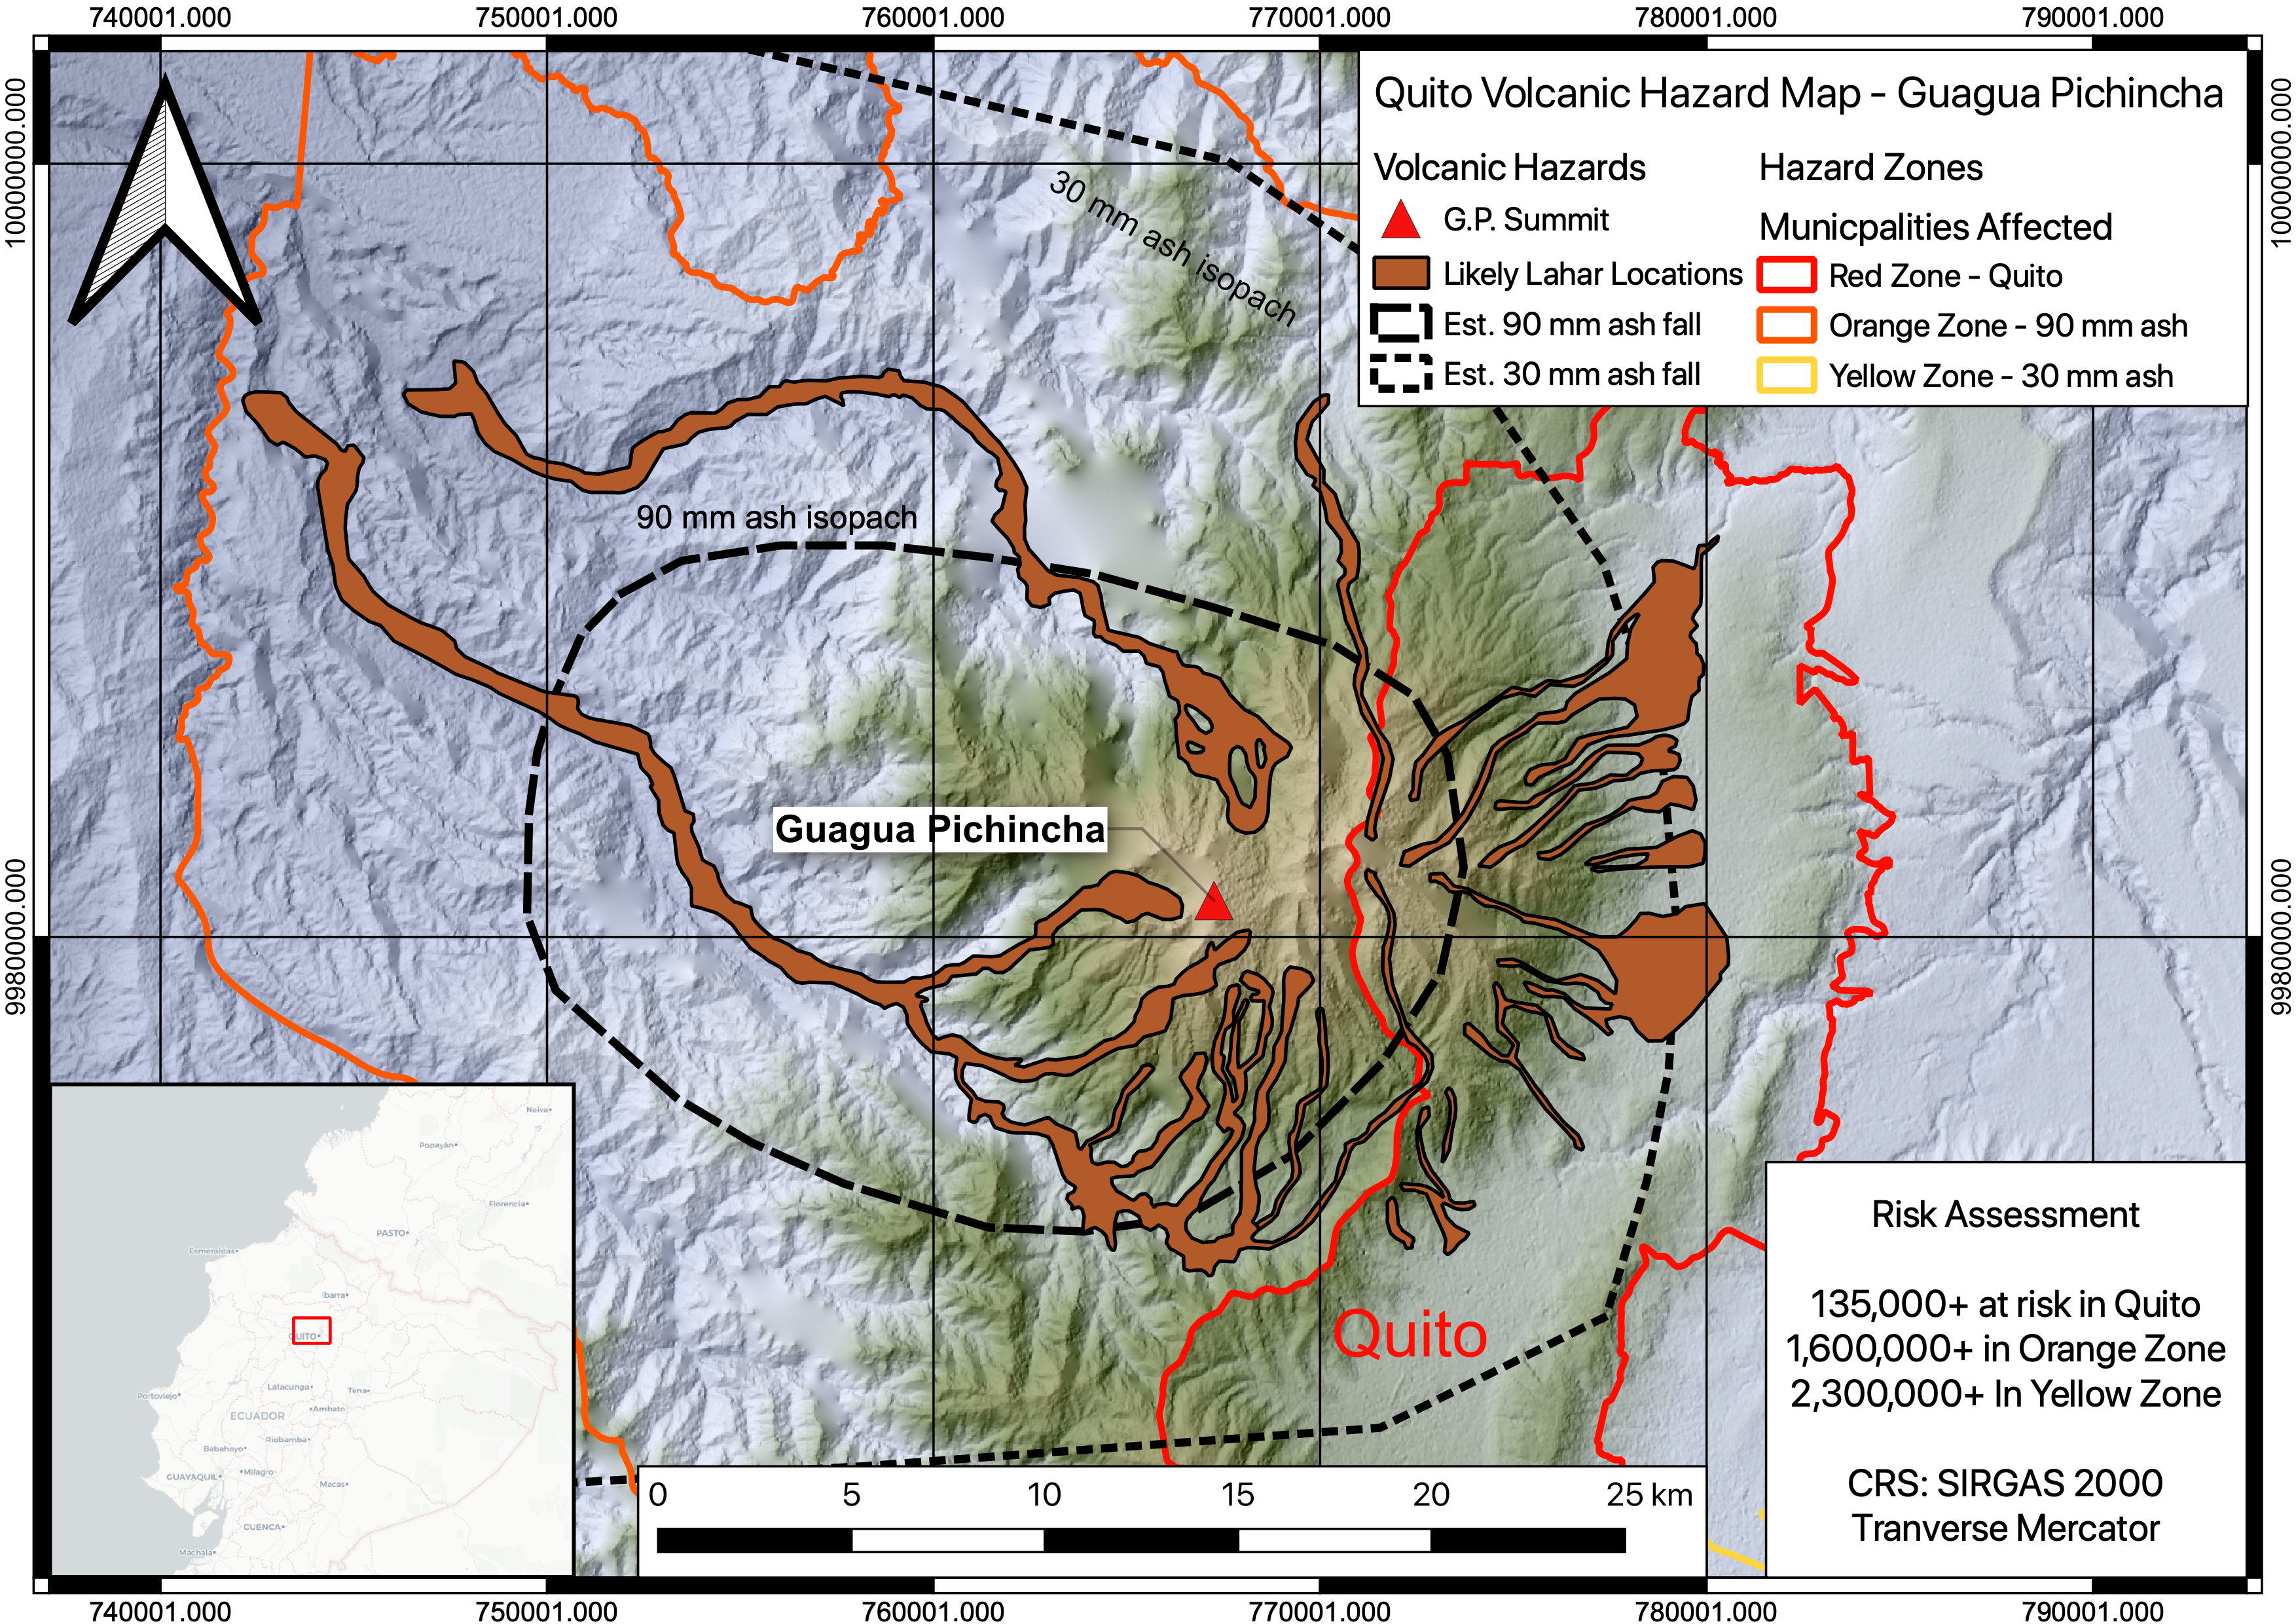
\includegraphics[width=0.9\textwidth]{Figure1_HazardMap_GP.png}
   \end{center}
\end{titlepage}

\tableofcontents

\section{Course Overview}

This guide was written in June of 2020 as an accompaniment to the "GIS for Dummies" workshop, organized by Catherine Crotty and Saraha Bodeving of McGill University (Canada). The workshop was presented in four parts, with the aim of introducing the use of Geographic Information Systems (GIS) to geoscientists in McGill's Society for Economic Geology (SEG) chapter. This section will provide a more general overview of the workshop, and preview the structure of the following guide, which is meant to accompany Part 2, Exercise 1. \textbf{All contents of this guide have been prepared by the course instructor, Nicholas Barber, and this guide can be shared under a MIT software License.} Feel free to share this guide and accompanying resources! \textit{Disclaimer: I (Nick Barber) claim no ownership of the data or underlying software used in this guide or this course.} 

This workshop was setup after preliminary discussions between myself, Catherine and Sarah throughout May 2020. In their role as organziers for their SEG chapter, they articulated a need to showcase what GIS is and what it can do for geoscientists. They wanted this course to include both a crash course for beginners, while also showcasing advanced features for more experienced users. Given the ongoing pandemic, the course was also to be hosted virtually. With these parameters in mind, I wrote an outline dividing our time into 4 blocks, to be spread over 4 days. Session 1 (Monday, June 15th) gave an overview lecture, covering the motivation for the course (Section XX), my background (see my web page), and the key theoretical material. The latter point as covered briefly, but ideally this topic will be given closer attention in a follow up GIS theory guide (this is a note to myself to write that, potentially for my undergrads). Wednesday June 17th saw Session 2, which in addition to this guide included a Lecture and a Live Demonstration of basic QGIS 3.10 functionality. The map on the title page is the desired output from Session 2. Session 3 will take place on Monday June 29th. The goal in this 2 hour block will be to run through some more advanced material, covering Python, spatial databases, mineral exploration (?) and style. Session 4 will be an open day where participants can schedule 1-1 thirty minute blocks with me, where I will advise them on their projects and the ways to get going with their particular analyses in GIS. 

The following sections will summarize Exercise 1, providing pictures with step by step details on how to replicate what I did in the live demo. I will start by briefly highlighting some of the goals and target skills in this demo. 

\subsection{Objectives}

The goal of this exercise to to familiarize users with the work flow of a typical GIS project.I wanted to show in (mostly) real time how you conceptualize a problem, find the data, set up the QGIS environment, conduct analyses, and export your desired output. I want this exercise to be both (1) an introduction to GIS project management and basic GIS analyses for users who may have never opened the program before, and (2) a refresher on basic GIS tasks, menus, and tools for more experienced users. 

\subsection{Target Skills}

% The notes for this section will be important for relating changes in magma composition, f\ce{O2}, and water content to changes in sulfur content. The sulfur content at sulfide saturation (SCSS) is in turn crucial for determining the distribution of metals between the melt and other competing reservoirs phases: sulfides, silicates, and volatiles. The sulfur model being considered here is the experimental model of \cite{jugo2009sulfur, jugo2010sulfur, Nash2019}. While this model is nearly a decade old, it does a good job accounting for conditions we are likely to encounter in relatively more oxidized melts. I'll support Jugo's models with observational evidence from \cite{richards2015oxidation}. Data to be used in the modeling will be recorded in a separate Excel file. 

% \cite{jugo2010sulfur} carries out a detailed XANES (X-Ray Absorption Near Edge Structure) spectroscopy on a population of synthetic basalts glasses and natural basaltic/basanitic samples from hotspot and arc environments (\cite{jugo2010sulfur}). The goal of the work was to provide 1) clarity regarding interpretation XANES measurements of S in igneous rocks and 2) models of S content and speciation as a function of fO2. For Jugo's experimental conditions, parameter space was fixed at P = 0.2 GPa (roughly 7 km depth), T = 1050\degree C, and composition set to a standard basalt (\cite{jugo2010sulfur}). This is about what we would expect in our arc condition space, but I will briefly discuss the advantages of \cite{Nash2019}'s more complex SCSS model that takes into account temperature and compositional effects on sulfide saturation. 

% After establishing the validity of their experiemntal and anaytical methods (see text for details), \cite{jugo2010sulfur} defines curves to fit a function to $S^{6+} / \Sigma S$ vs. fO2 :

% \begin{equation} \label{Jugo_eq10}
% \mathrm{S}^{6+} / \Sigma \mathrm{S}=1 /\left(1+10^{(2.1-2 \Delta \mathrm{FMQ})}\right)
% \end{equation}


\section{Project Panning}

\section{Finding GIS Data}

\section{Importing Data}

\subsection{Vector}

\subsection{Raster}

\subsection{CSV}

\section{Defining Coordinate Systems and Projections}

\section{Reprojection}

\section{Setting Up Workspace}

\section{Georeferencing Our Base Map}

\section{Tracing New Features}

\section{Accounting for errors}

\section{Analysis}

\subsection{Field Calculator}

\subsection{Geoprocessing}

\subsection{Statistics Viewer}

\section{Symbology}

\subsection{3D View}

\section{Layout Manager}

\section{Final Thoughts}

\section{Data Sources and Further Reading}

\section{Acknowledgements}

\newpage
\printbibliography

\end{document}
